\documentclass[10pt]{beamer}
\usepackage[utf8]{inputenc}
\usepackage[english,russian]{babel}
\usepackage{beamerthemesplit}
\usepackage{amsmath,amssymb,amsfonts,amsthm,mathtext}
\usepackage{graphicx,psfrag} %only include if using pictures with psfrag

\usetheme{Warsaw}
\usecolortheme{Marcusmae}

\title[Схема переноса MPDATA]{Масштабируемая массивно-параллельная реализация схемы переноса примесей MPDATA на распределенных GPU/SMP системах}
\author{Левченко Олег --  Петров Артем -- Микушин Дмитрий}
\institute{Геофизический Центр РАН -- СибНИГМИ РАН -- ИВМ РАН}
\date{октябрь, 2010}



\begin{document}

\setbeamertemplate{title page}[default][rounded=true,shadow=false]
\setbeamertemplate{background canvas}{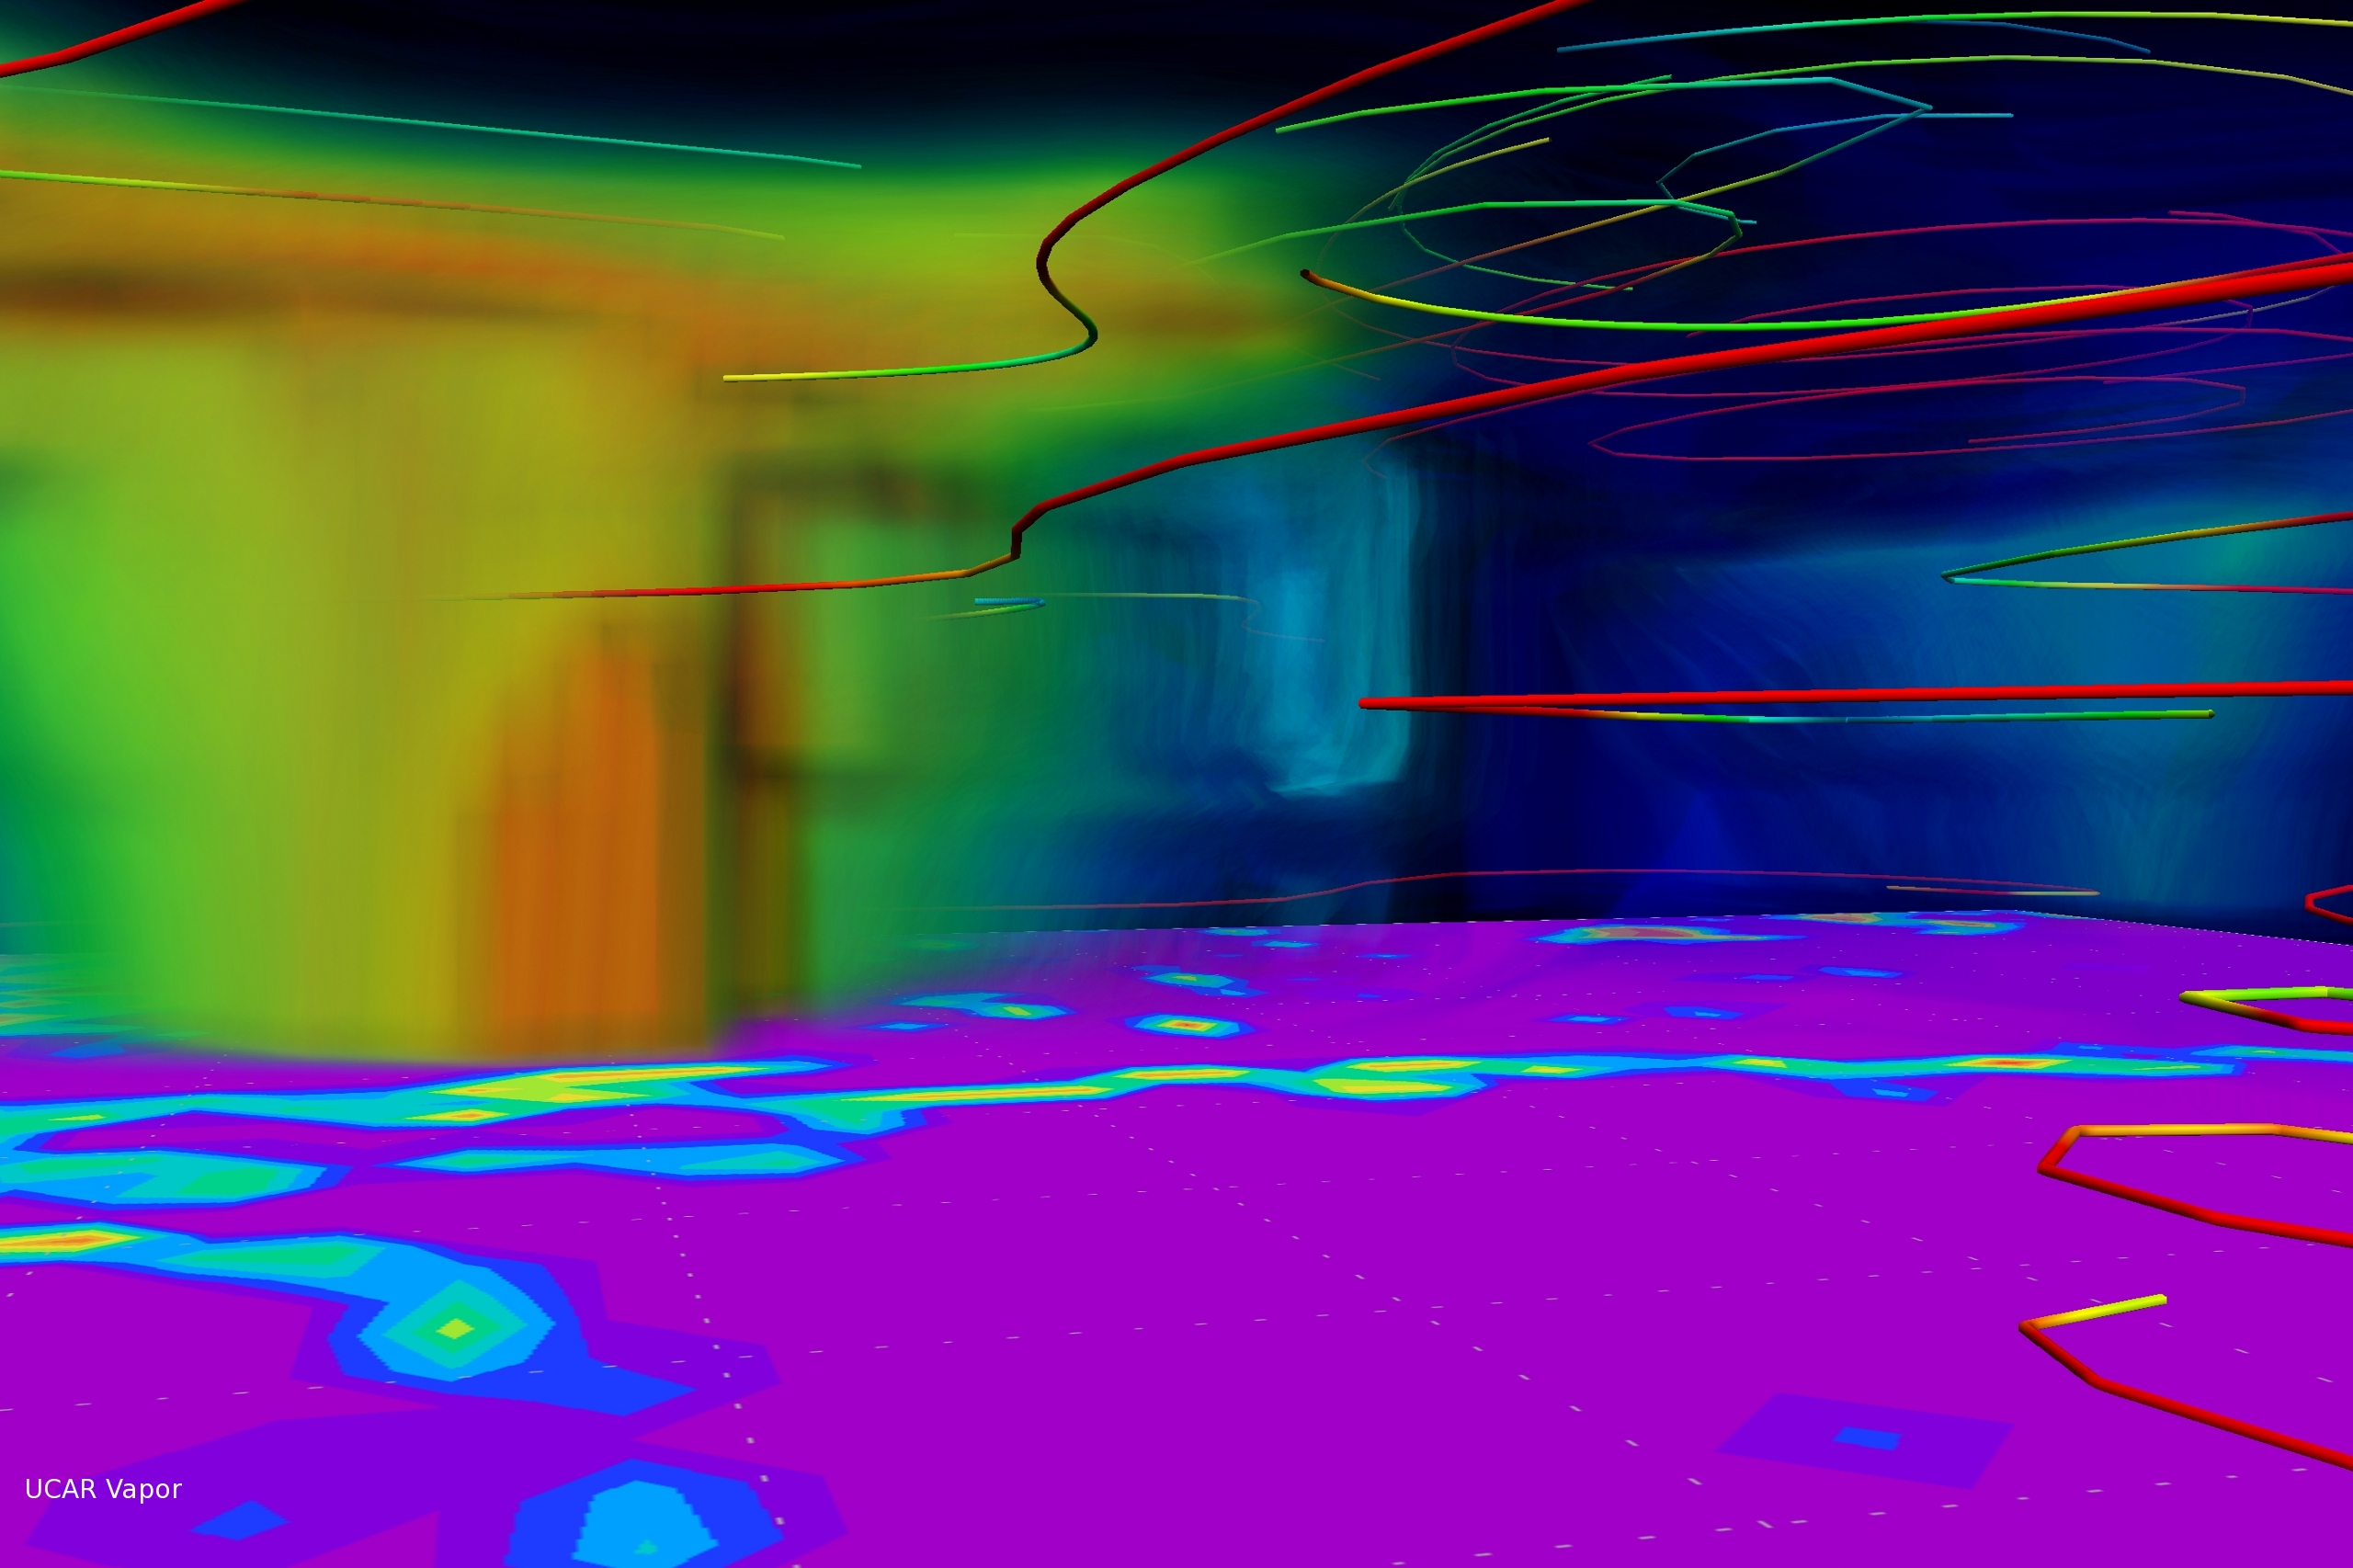
\includegraphics[height=\paperheight]{artwork/images/front}}

\begin{frame}
\titlepage
\end{frame}

\setbeamertemplate{background canvas}{}

\begin{frame}{План}
\begin{itemize}
\item[•] Физическая задача
\item[•] Выбор численного метода
\item[•] Численная схема MPDATA
\item[•] Проект параллельной реализации MPDATA для гибридных суперкомпьютеров
\begin{itemize}
\item[o] Общая схема вычислений
\item[o] Архитектура GPU GT200
\item[o] Анализ реализации для GPU
\item[o] Метод декомпозиции прямоугольной сетки
\end{itemize}
\item[•] Заключение
\end{itemize}
\end{frame}

\begin{frame}{Перенос примеси как физическая задача}
\begin{picture}(0.0,0.0)
\put(-20,-55){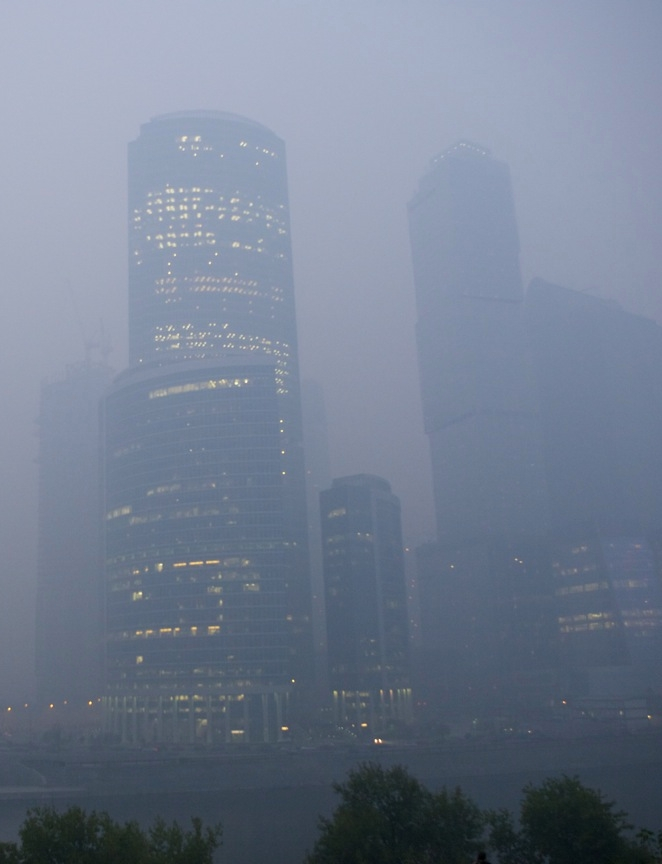
\includegraphics[height=2.7cm]{artwork/images/moscow}}
\end{picture}
\begin{picture}(0.0,0.0)
\put(43,-55){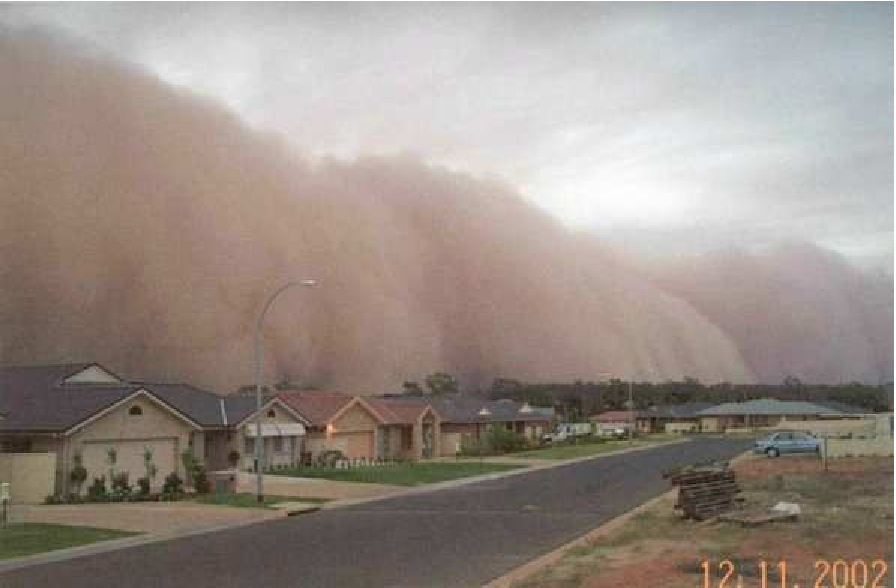
\includegraphics[height=2.7cm]{artwork/pdf/dust}}
\end{picture}
\begin{picture}(0.0,0.0)
\put(165,-55){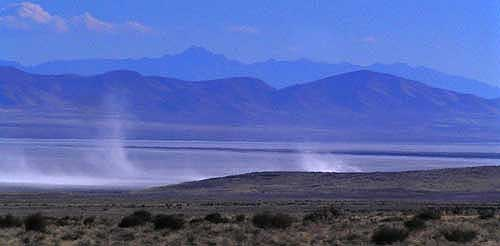
\includegraphics[height=2.7cm]{artwork/images/salt}}
\end{picture}

\vskip 78pt
\begin{itemize}
\item[•]Тип источника (точечный, распределённый)
\item[•]Тип аэрозоля (пепел, песок, соль, ...)
\item[•]Распределение размеров частиц (мониторинг концентрации опасной мелкодисперсной пыли)
\item[•]Динамика: эмиссия (+ сальтация), перенос (+ химические процессы), осаждение
\end{itemize}
\end{frame}

\begin{frame}{Модели и численные схемы}
\begin{itemize}
  \item Физические уравнения модели прогноза погоды WRF v.3 \cite{wrf:arw}
  \item Численные схемы адвекции
\begin{itemize}
  \item Ориентированы на пассивные примеси
  \item Сохранение массы
  \item Эйлеровы модели
    \begin{itemize}
    \item Ограничения на временной шаг
    \end{itemize}
  \item Полу-Лагранжевые модели:
    \begin{itemize}
    \item Большие временные шаги без потери стабильности
    \item Порядок точности
    \item Сохранение массы/положительно-определенность
    \item Overshooting/undershooting
  \end{itemize}
\end{itemize}

\end{itemize}



\begin{figure}
\centering
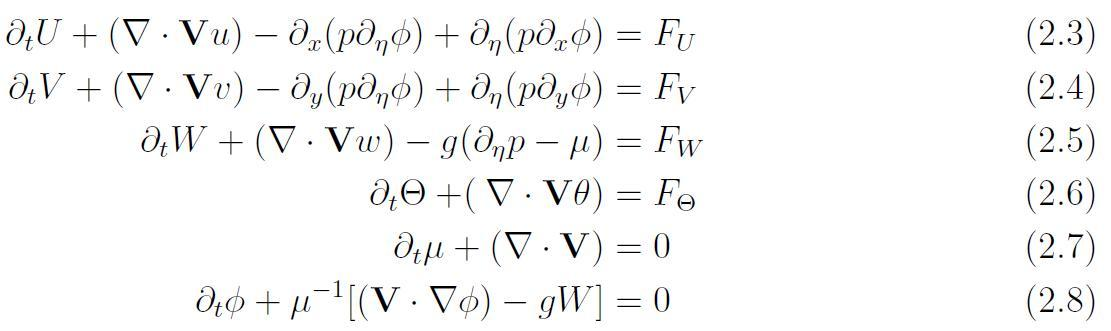
\includegraphics[height=1in, width=3in]{artwork/images/wrf_governing_equations}
\label{fig:wrf-equations}
\end{figure}

\end{frame}



\begin{frame}{Характерные особенности MPDATA}
Специально разработана под метеорологические нужды:
\begin{itemize}
  \item Положительная определенность
  \item Сохранение массы
  \item Вычислительная простота, сравнимая с донорной схемой
\end{itemize}
\end{frame}


\begin{frame}{Расширения MPDATA}
Численная модель вычислений MPDATA хорошо теоретически проработана и включает следующие расширения \cite{smolar:mpdata-solver}:
\begin{itemize}
  \item Возможность увеличить пространственную точность до третьего порядка, временную точность до пятого
  \item Возможность эмпирической подстройки для увеличения точности без увеличения вычислительной сложности
  \item Физическая диффузия в составе адвективного потока
  \item Траспорт скалярного поля с переменным знаком
  \item Моделирование дивергентных полей
\end{itemize}
\end{frame}

\begin{frame}{Почему MPDATA?}
\begin{itemize}
\item Численная модель вычислений MPDATA потенциально может быть оптимизирована под CUDA:
\begin{itemize}
  \item Соотношение доступов в память к вычислениям
  \item Явная модель вычислений
\end{itemize}
  \item Является частью численных гидродинамических моделей погоды EULAG и NH3D
\end{itemize}
\end{frame}



\begin{frame}{Одномерный случай - формулировка адвекции\cite{smolar:mpdata-1d}}

\begin{enumerate}
  \item $ \frac{\partial \Psi}{\partial t} + \frac{\partial (\Psi \cdot \upsilon)}{\partial x} = 0 $, где $\Psi$ - концентрация, $\upsilon$ - скорость ветра
  \item $ \Psi^{n+1}_i = \Psi^{n}_i + [\overbrace{F(\Psi^{n}_{i-1}, \Psi^{n}_{i}, U^{n+1/2}_{i-1/2})}^\text{входной поток} - \overbrace{F(\Psi^{n}_{i}, \Psi^{n}_{i+1}, U^{n+1/2}_{i+1/2})}^\text{выходной поток}] $
  \item $F(\Psi_L, \Psi_R, U)=0.5\cdot(U+|U|)\cdot \Psi_L + 0.5\cdot(U-|U|)\cdot \Psi_R$, где $U=\upsilon \cdot \frac{\Delta t}{\Delta x}$
  \item $\underset{i, n}{\max}|\upsilon_{i\pm1/2}|\cdot \frac{\Delta t}{\Delta x}\leqslant1$ - условие стабильности схемы
  \item $O(\Delta x)$ - недостаточно для практических применений
\end{enumerate}

\end{frame}



\begin{frame}{Одномерный случай - MPDATA\cite{smolar:mpdata-1d}}

\begin{enumerate}
  \item $ \frac{\partial \Psi_{i}^{n}}{\partial t} + \frac{\partial (\Psi_{i}^{n} \cdot \upsilon)}{\partial x} = \frac{\partial [\frac{1}{2}\cdot(|\upsilon|\cdot \Delta x - \upsilon^2\cdot \Delta t)\cdot \frac{\partial \Psi_{i}^{n}}{\partial x}]}{\partial x}  $ вместо
      $ \frac{\partial \Psi_{i}^{n}}{\partial t} + \frac{\partial (\Psi_{i}^{n} \cdot \upsilon)}{\partial x} = 0$
  \item $ \frac{\partial \Psi}{\partial t} + \frac{\partial (\Psi \cdot \upsilon)}{\partial x} = \frac{\partial (K\cdot \frac{\partial \Psi}{\partial x})}{\partial x} $ где $K=\frac{1}{2}\cdot(|\upsilon|\cdot \Delta x - \Delta t \cdot \upsilon^2)$ - коэффициент диффузии
  \item $ \frac{\partial \Psi}{\partial t} -  \frac{\partial (K\cdot \frac{\partial \Psi}{\partial x})}{\partial x} = 0$ - "скрытое" уравнение адвекции
  \item $ \frac{\partial \Psi}{\partial t} +  \frac{\partial (\Psi \cdot \upsilon_{diff})}{\partial x} = 0$ где $\upsilon_{diff}=-\frac{K}{\Psi}\cdot \frac{\partial \Psi}{\partial x}$
  \item $u_{antidiff} = -u_{diff}$ - "проигрыш" диффузии назад во времени 
  \item $ \Psi^{*}_i = \Psi^{n}_i + [F(\Psi^{n}_{i-1}, \Psi^{n}_{i}, U^{n+1/2}_{i-1/2}) - F(\Psi^{n}_{i}, \Psi^{n}_{i+1}, U^{n+1/2}_{i+1/2})] $
  \item $ \Psi^{n+1}_i = \Psi^{*}_i + [F(\Psi^{*}_{i-1}, \Psi^{*}_{i}, \upsilon^{antidiff}_{i-1/2}) - F(\Psi^{*}_{i}, \Psi^{*}_{i+1}, \upsilon^{antidiff}_{i+1/2})] $ где $\upsilon_{i+1/2}^{antidiff}=\frac{(|\upsilon_{i+1/2}|\cdot \Delta x - \Delta t\cdot \upsilon^{2}_{i+1/2})\cdot(\Psi^{*}_{i+1}-\Psi^{*}_{i})}{(\Psi^{*}_{i}+\Psi^{*}_{i+1}+\epsilon)\cdot \Delta x}$
  \item $O(\Delta x^2)$ - достаточно для практических применений
\end{enumerate}

\end{frame}


%\begin{frame}{Произвольная размерность}

\[ \frac{\partial G\cdot\psi}{\partial t} + \nabla \cdot (\upsilon \cdot \psi) = G \cdot R \]



\end{frame}


\begin{frame}{Целевая гибридная вычислительная система}

\begin{figure}
\centering
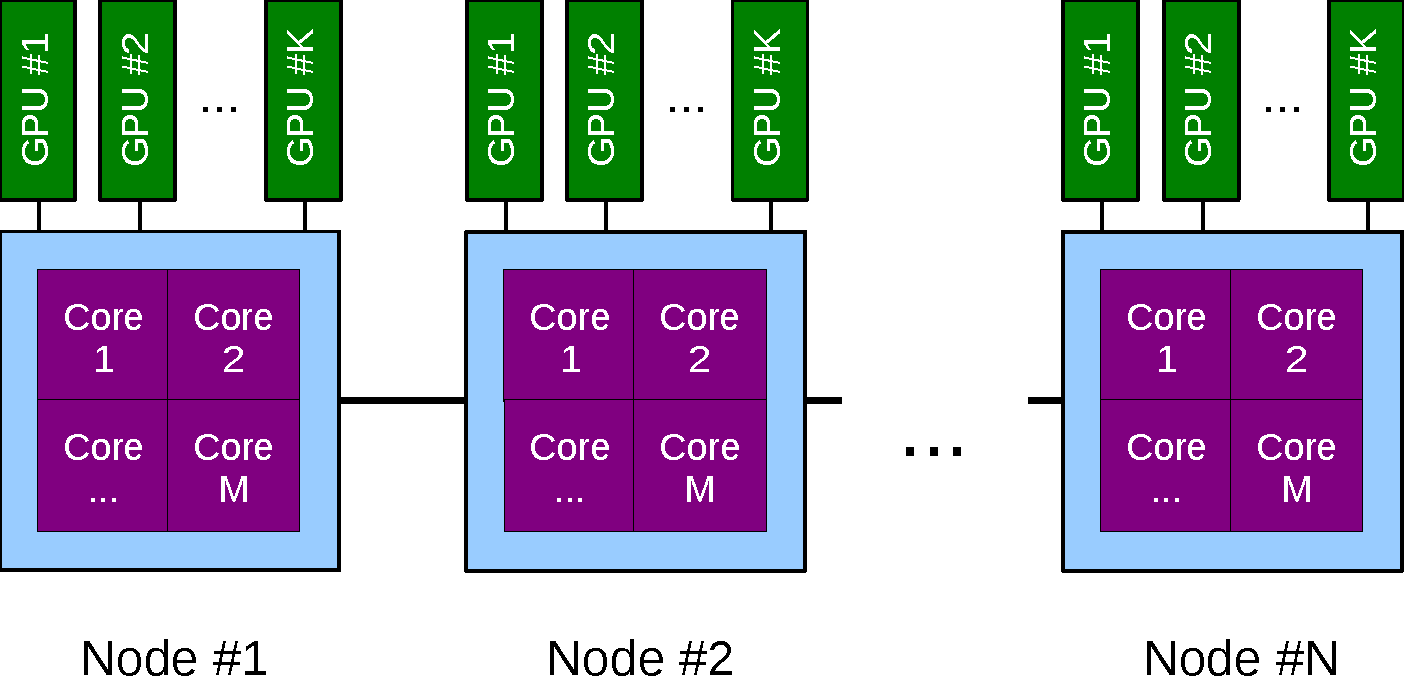
\includegraphics[width=4.2in]{artwork/pdf/hybrid_scheme}
\end{figure}

\end{frame}



\begin{frame}{Структура GPU-CPU программного комплекса\cite{maemarcus:diploma}}

\begin{figure}
\centering
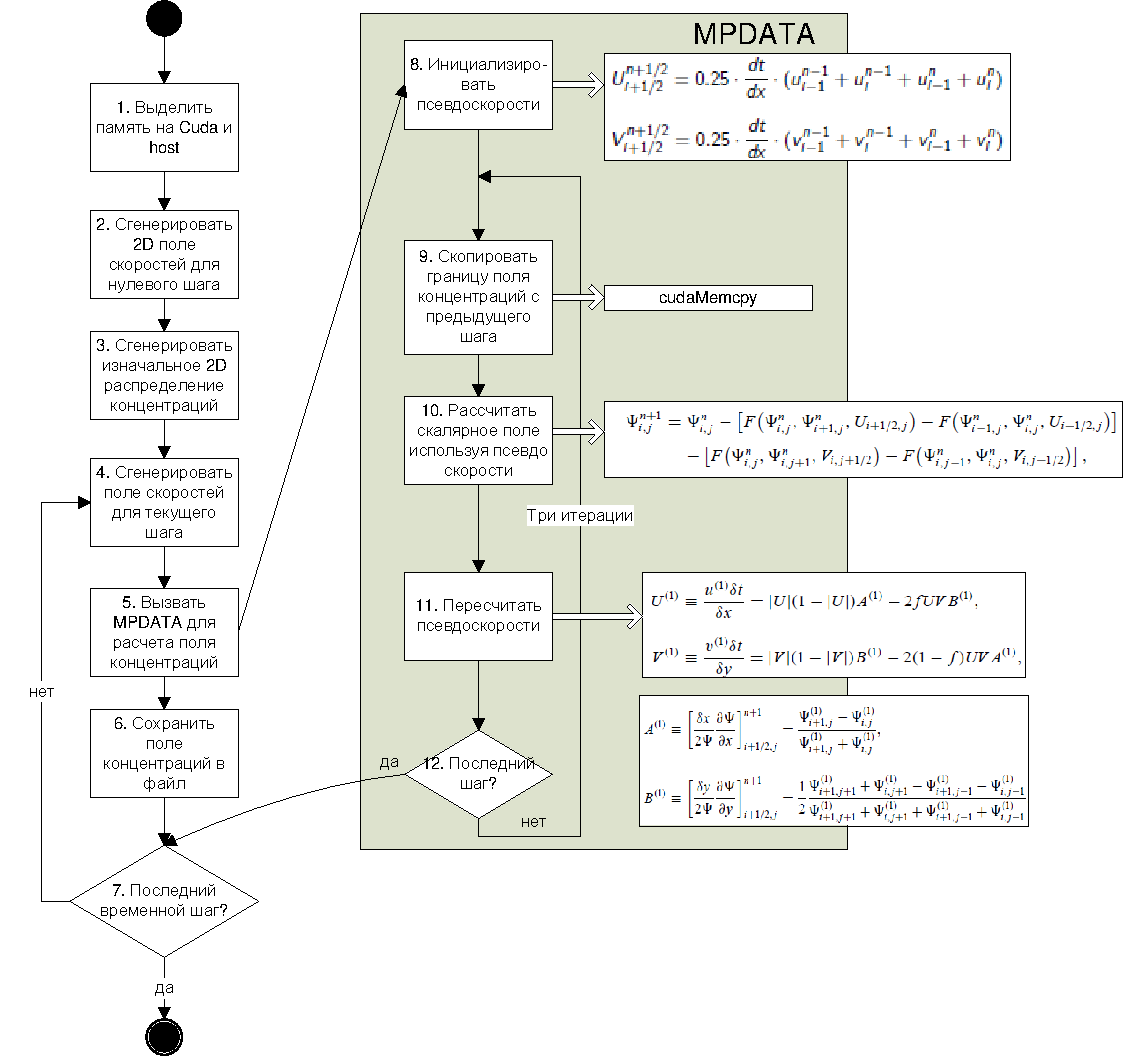
\includegraphics[height=3.1in, width=3in]{artwork/pdf/code}
\label{fig:wrf-equations}
\end{figure}

\end{frame}




\begin{frame}{GPGPU - Кластер из мультипроцессоров\cite{web:rwgpu}}

\begin{itemize}
  \item Асинхронные вычислительные мультипроцессоры
  \item Общая многопортовая память
  \item Конвейеры текстурной памяти
\end{itemize}



\begin{figure}
\centering
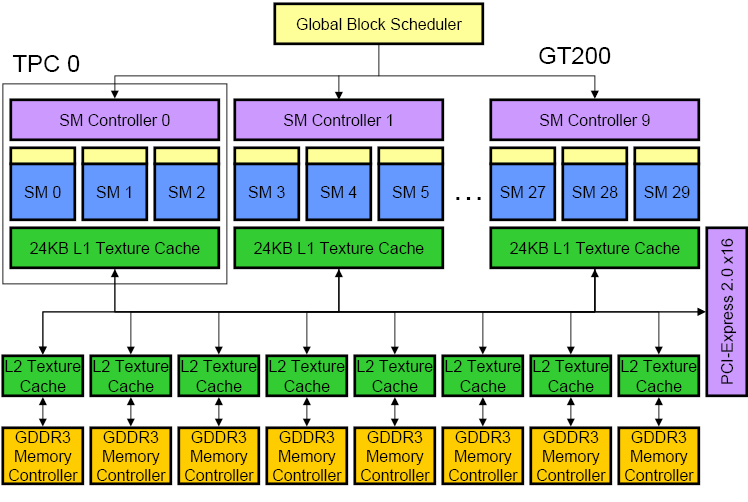
\includegraphics[height=2in, width=3in]{artwork/images/board}
\label{fig:board}
\end{figure}

\end{frame}

\begin{frame}{Мультипроцессор GT 200\cite{web:rwgpu}}
\begin{itemize}
  \item WARP и \_\_syncthreads()
  \item Треугольник "регистры - разделяемая память - потоки"
  \item Специфичные оптимизации по паттернам доступа к памяти
\end{itemize}



\begin{figure}
\centering
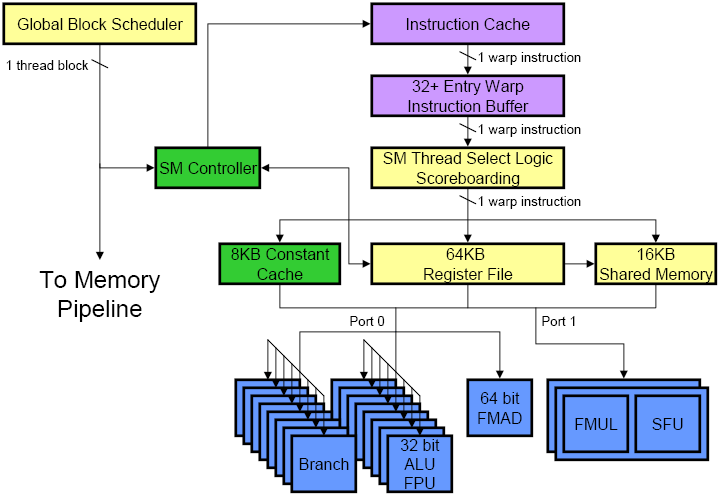
\includegraphics[height=2in, width=3in]{artwork/images/SM}
\label{fig:sm}
\end{figure}

\end{frame}


\begin{frame}{Dual Issue\cite{web:rwgpu}}
\begin{itemize}
  \item Двойное опережение
  \item Зависимости между 64-bit fpu и 32-bit fpu
\end{itemize}



\begin{figure}
\centering
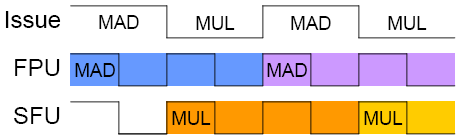
\includegraphics[height=2in, width=3in]{artwork/images/dual_issue}
\label{fig:dual_issue}
\end{figure}

\end{frame}


\begin{frame}{Инициализация псевдоскоростей на CUDA}

\begin{figure}
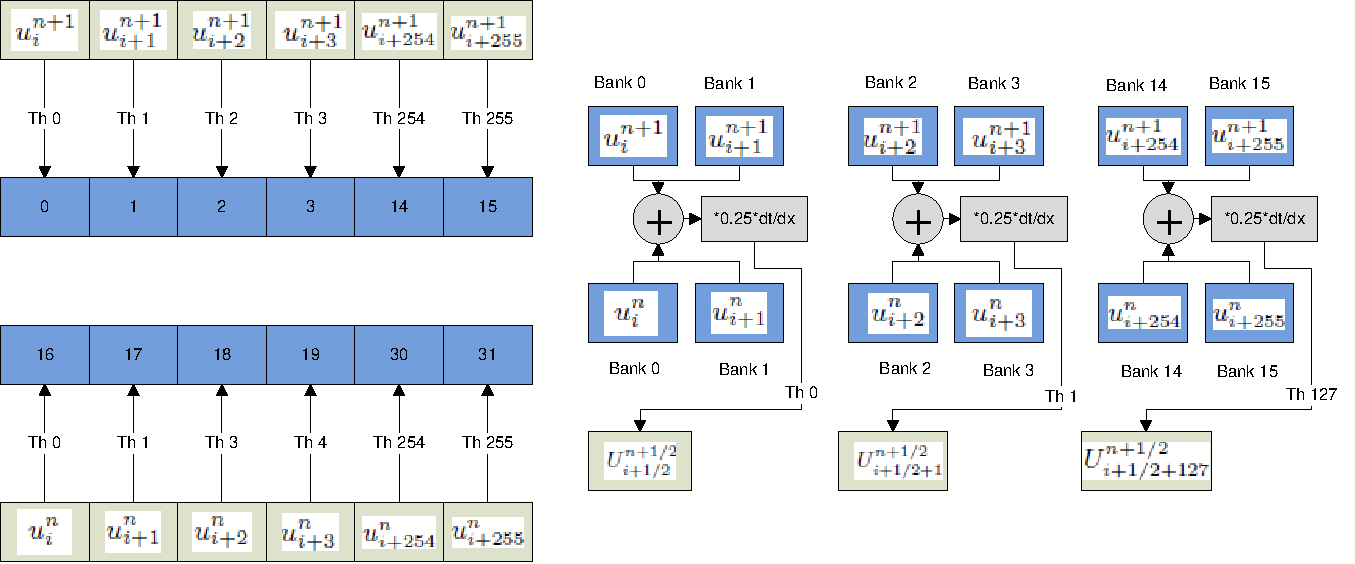
\includegraphics[height=2in, width=3.5in]{artwork/pdf/uu_init}
\label{fig:wrf-equations}
\end{figure}

\[ U^{n+1/2}_{i+1/2}=0.25 \cdot \frac{dt}{dx} \cdot(u^{n-1}_{i-1} + u^{n-1}_{i} + u^{n}_{i-1} + u^{n}_{i}) \]


\begin{itemize}
  \item Склейка по доступу в глобальную память (Coalescing)
  \item Эффективная блокировка варпов (Warps Stall)
  \item Возможен двухкратный конфликт по банкам разд. памяти
\end{itemize}

\end{frame}

\begin{frame}{Анализ производительности мультипроцессора\cite{kirk:cuda}}
\begin{enumerate}
  \item Загрузка $\upsilon^{n+1}_{i+0+..255}$
  \begin{itemize}
        \item $N_{threads}=256 \Rightarrow N_{warps}=\frac{256}{32}=8$ 
        \item $ShMemSize_1 = N_{threads}\cdot 2 \cdot 4 = 2048$ Bytes
  \end {itemize}
  \item Загрузка $\upsilon^{n}_{i+0+..255}$
  \begin{itemize}
        \item $N_{threads}=256 \Rightarrow N_{warps}=\frac{256}{32}=8$
        \item $ShMemSize_2 = N_{threads}\cdot 2 \cdot 4 = 2048$ Bytes
  \end {itemize}
  \item Вычисление $U^{n+1/2}_{i+1/2+..127}$
  \begin{itemize}
        \item $N_{threads}=\frac{256}{2}=128 \Rightarrow N_{warps}=\frac{128}{32}=4$
  \end {itemize}
  \item Анализ загрузки мультипроцессора
  \begin{itemize}
   \item Максимальное количество блоков на мультипроцессоре по потокам $MaxBlocks_{threads}=\frac{1024}{256}=4$
   \item Максимальное количество блоков на мультипроцессоре по разделяемой памяти $MaxBlocks_{shmem}=\frac{MaxShmem}{ShMemSize_1 + ShMemSize_2}=\frac{32768}{2048 + 2048}=8$
  \end {itemize}
  \item Вывод - так как алгоритм memory-bound, то фактором, сдерживающим производительность мультипроцессора, может стать нехватка регистров, если $N_{regs}\gtrdot \frac{16384}{1024}=16$
\end{enumerate}
\end{frame}


\begin{frame}{Дублирование границ при декомпозиции}

\begin{figure}
\centering
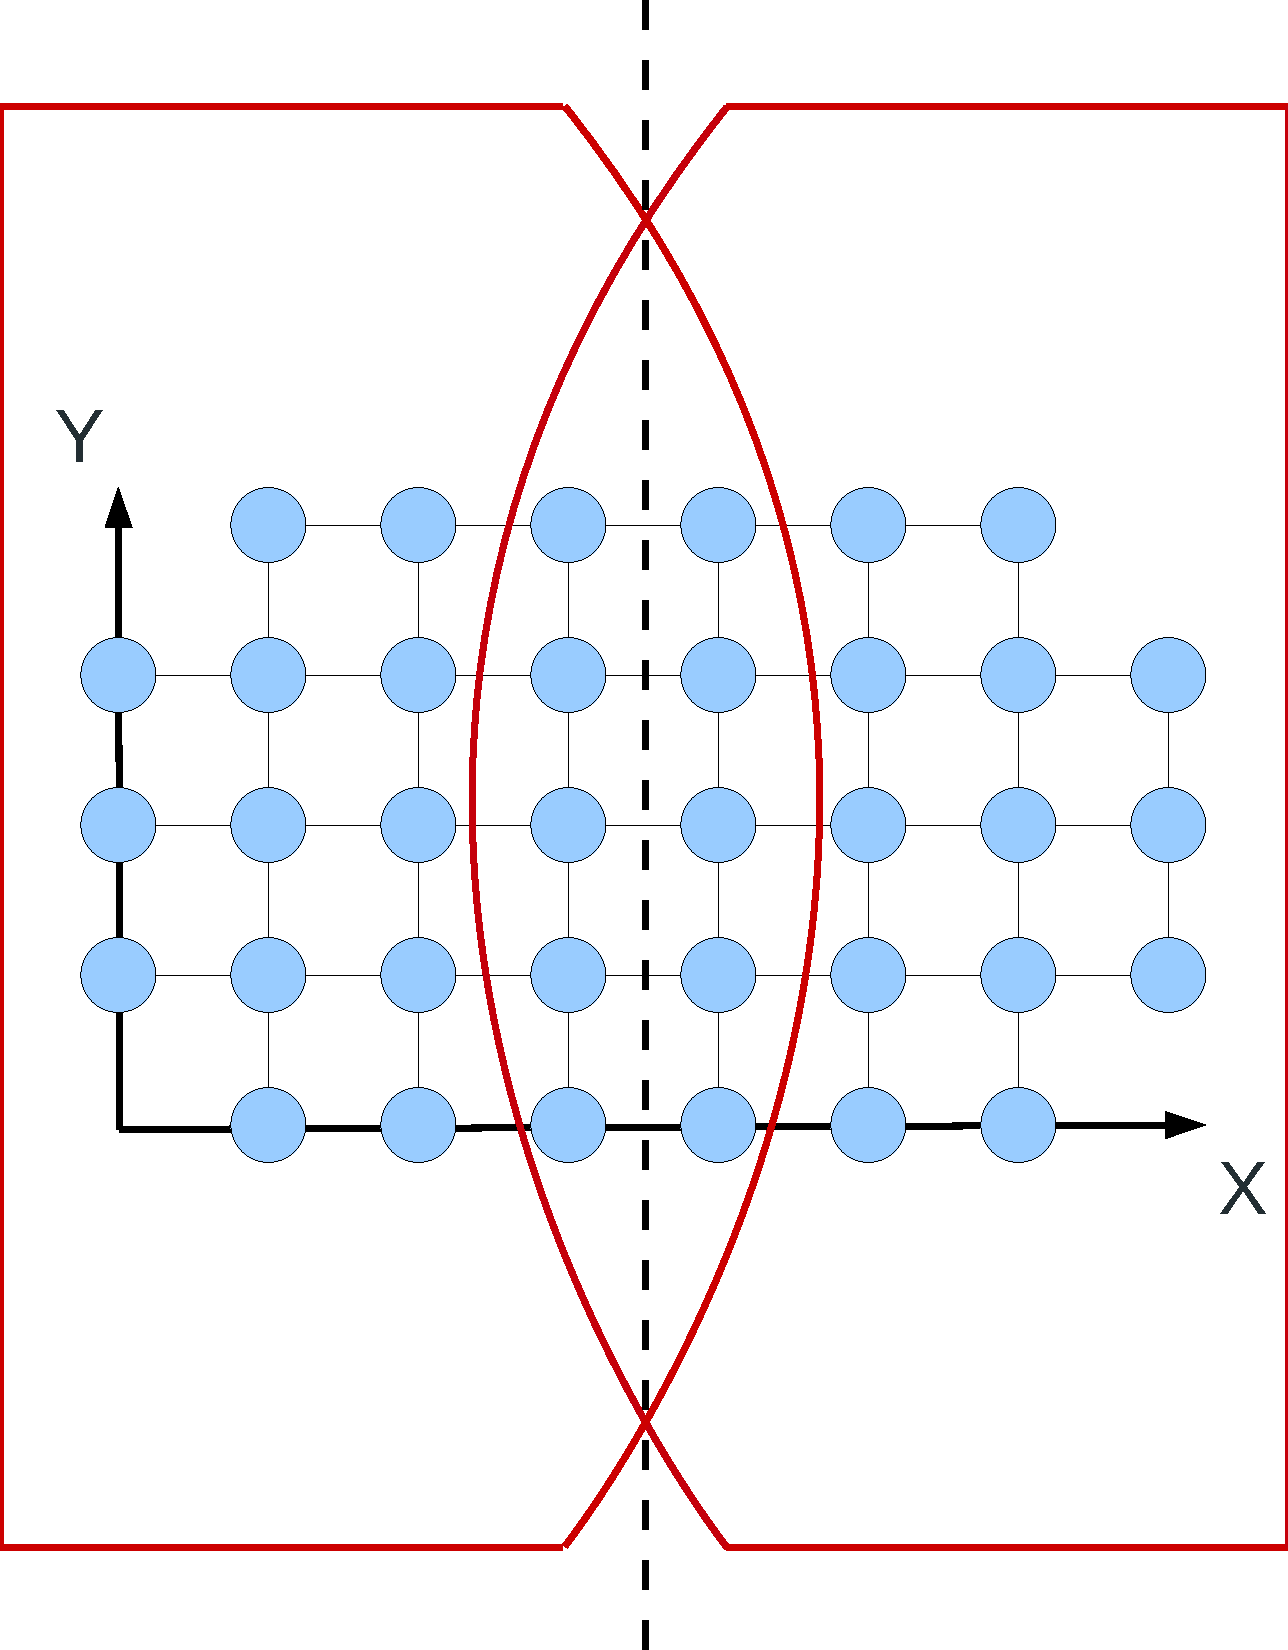
\includegraphics[height=2.5in]{artwork/pdf/decomp_0}
\end{figure}

\end{frame}

\begin{frame}{Данные в распределённой памяти}

\begin{figure}
\centering
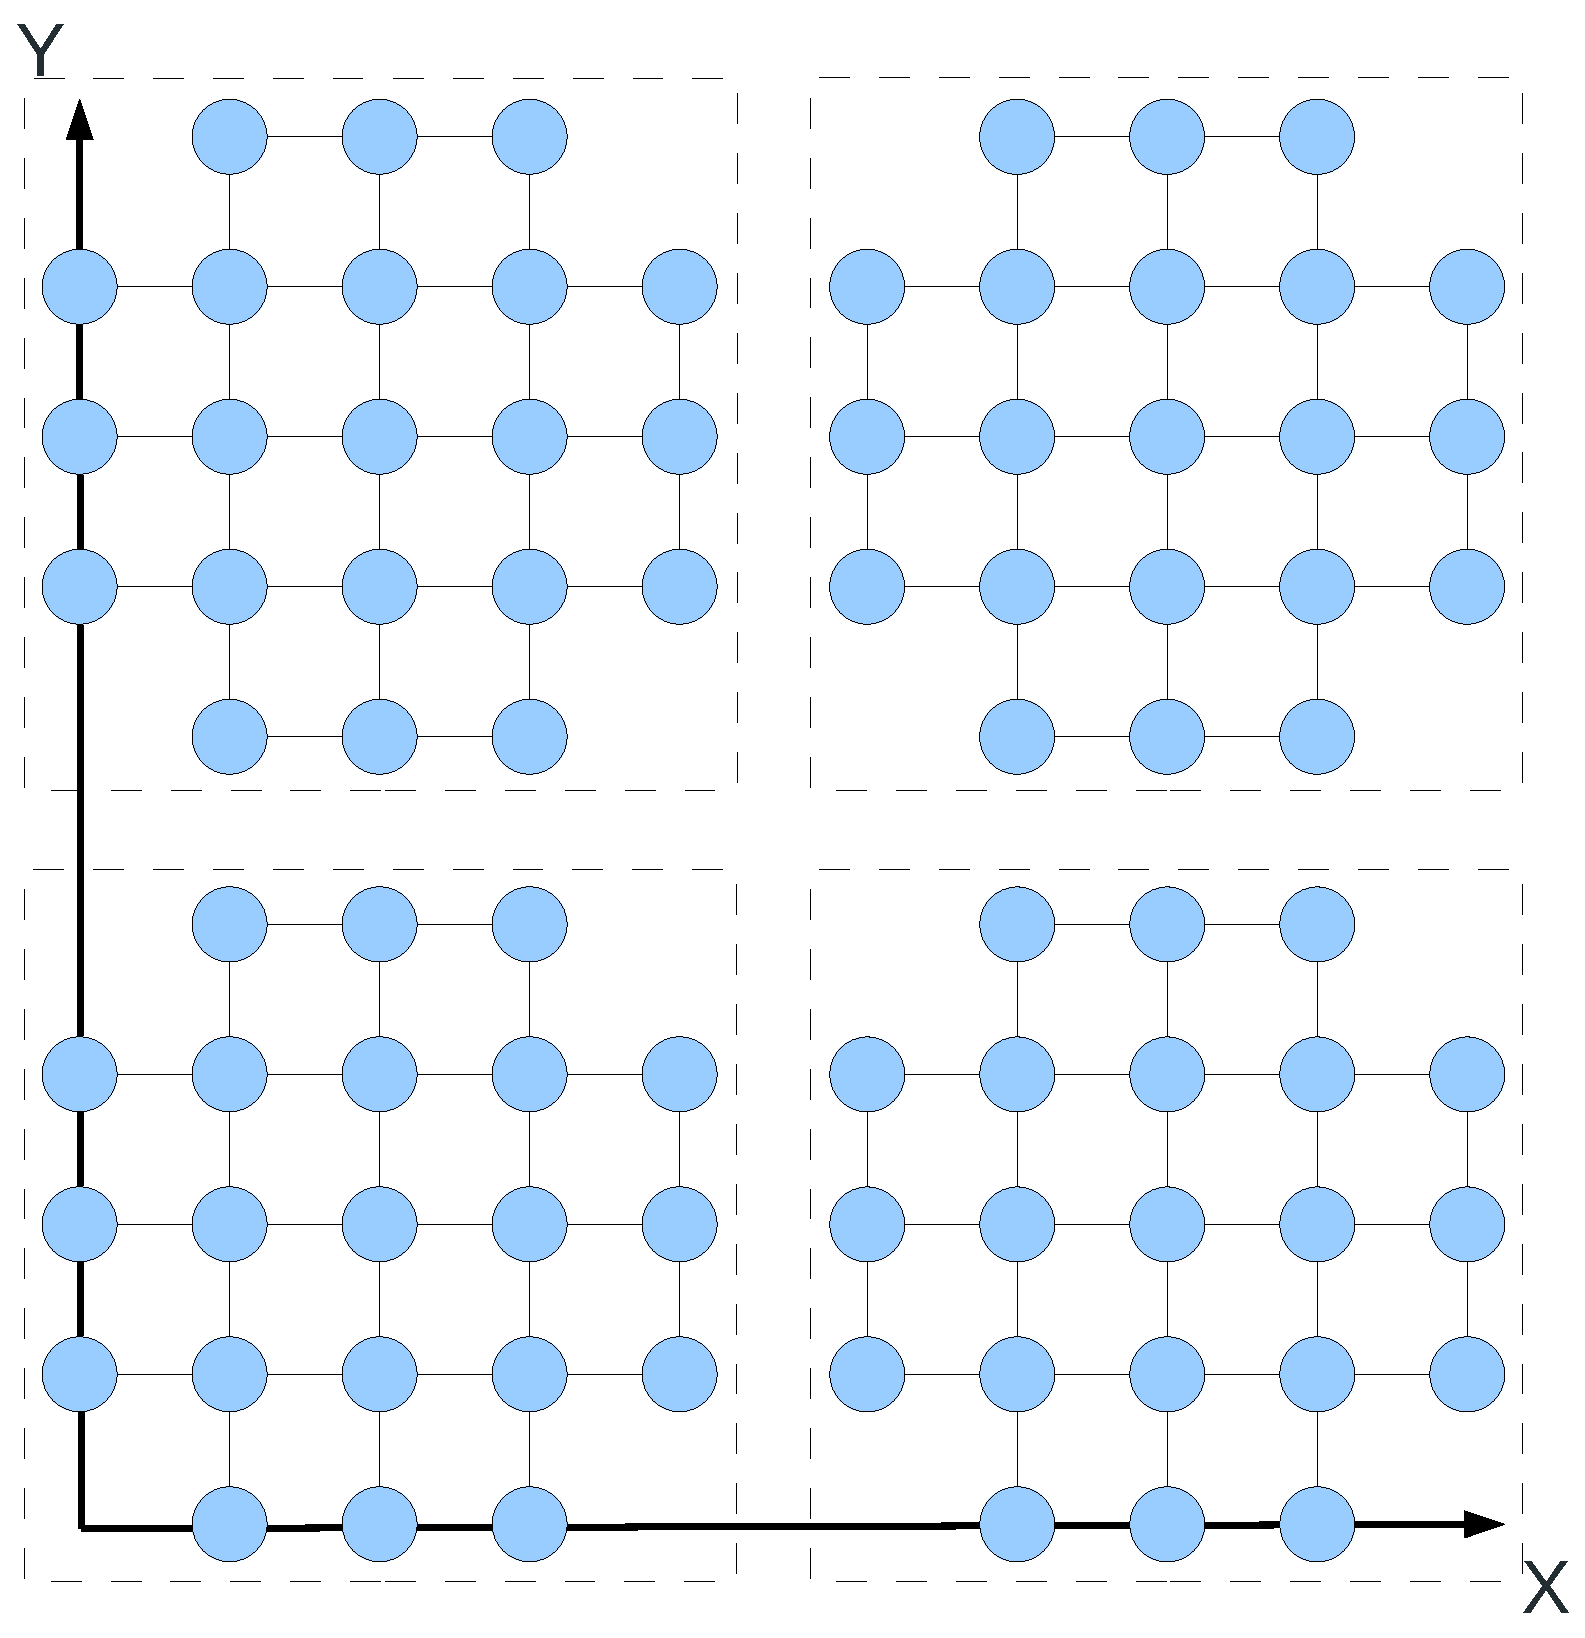
\includegraphics[height=2.5in]{artwork/pdf/decomp_1}
\end{figure}

\end{frame}

\begin{frame}{Параллельный расчёт внутренних узлов}

\begin{figure}
\centering
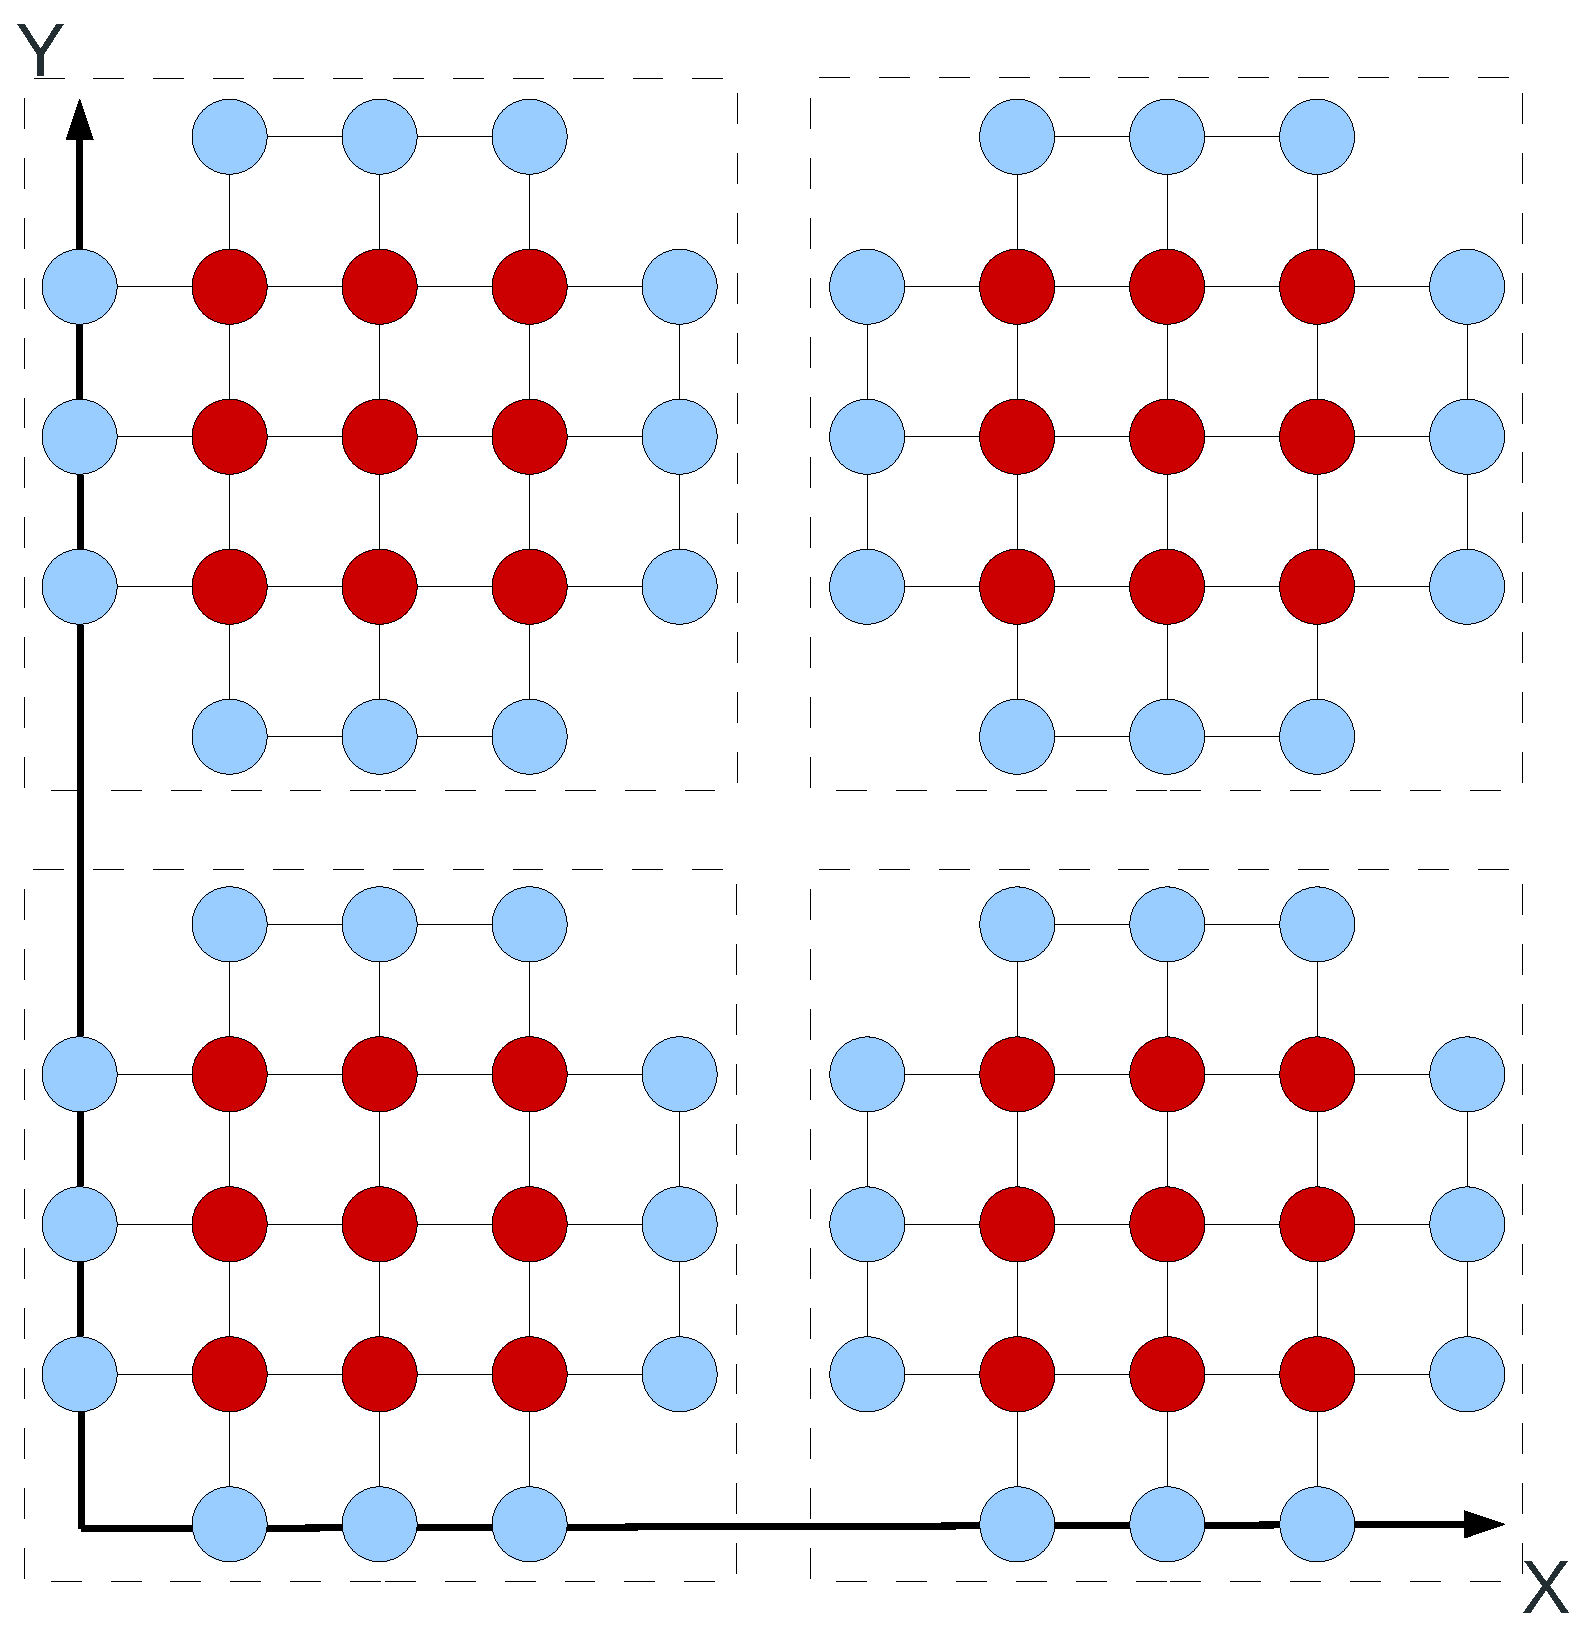
\includegraphics[height=2.5in]{artwork/pdf/decomp_2}
\end{figure}

\end{frame}


\begin{frame}{Синхронизация граничных узлов}

\begin{figure}
\centering
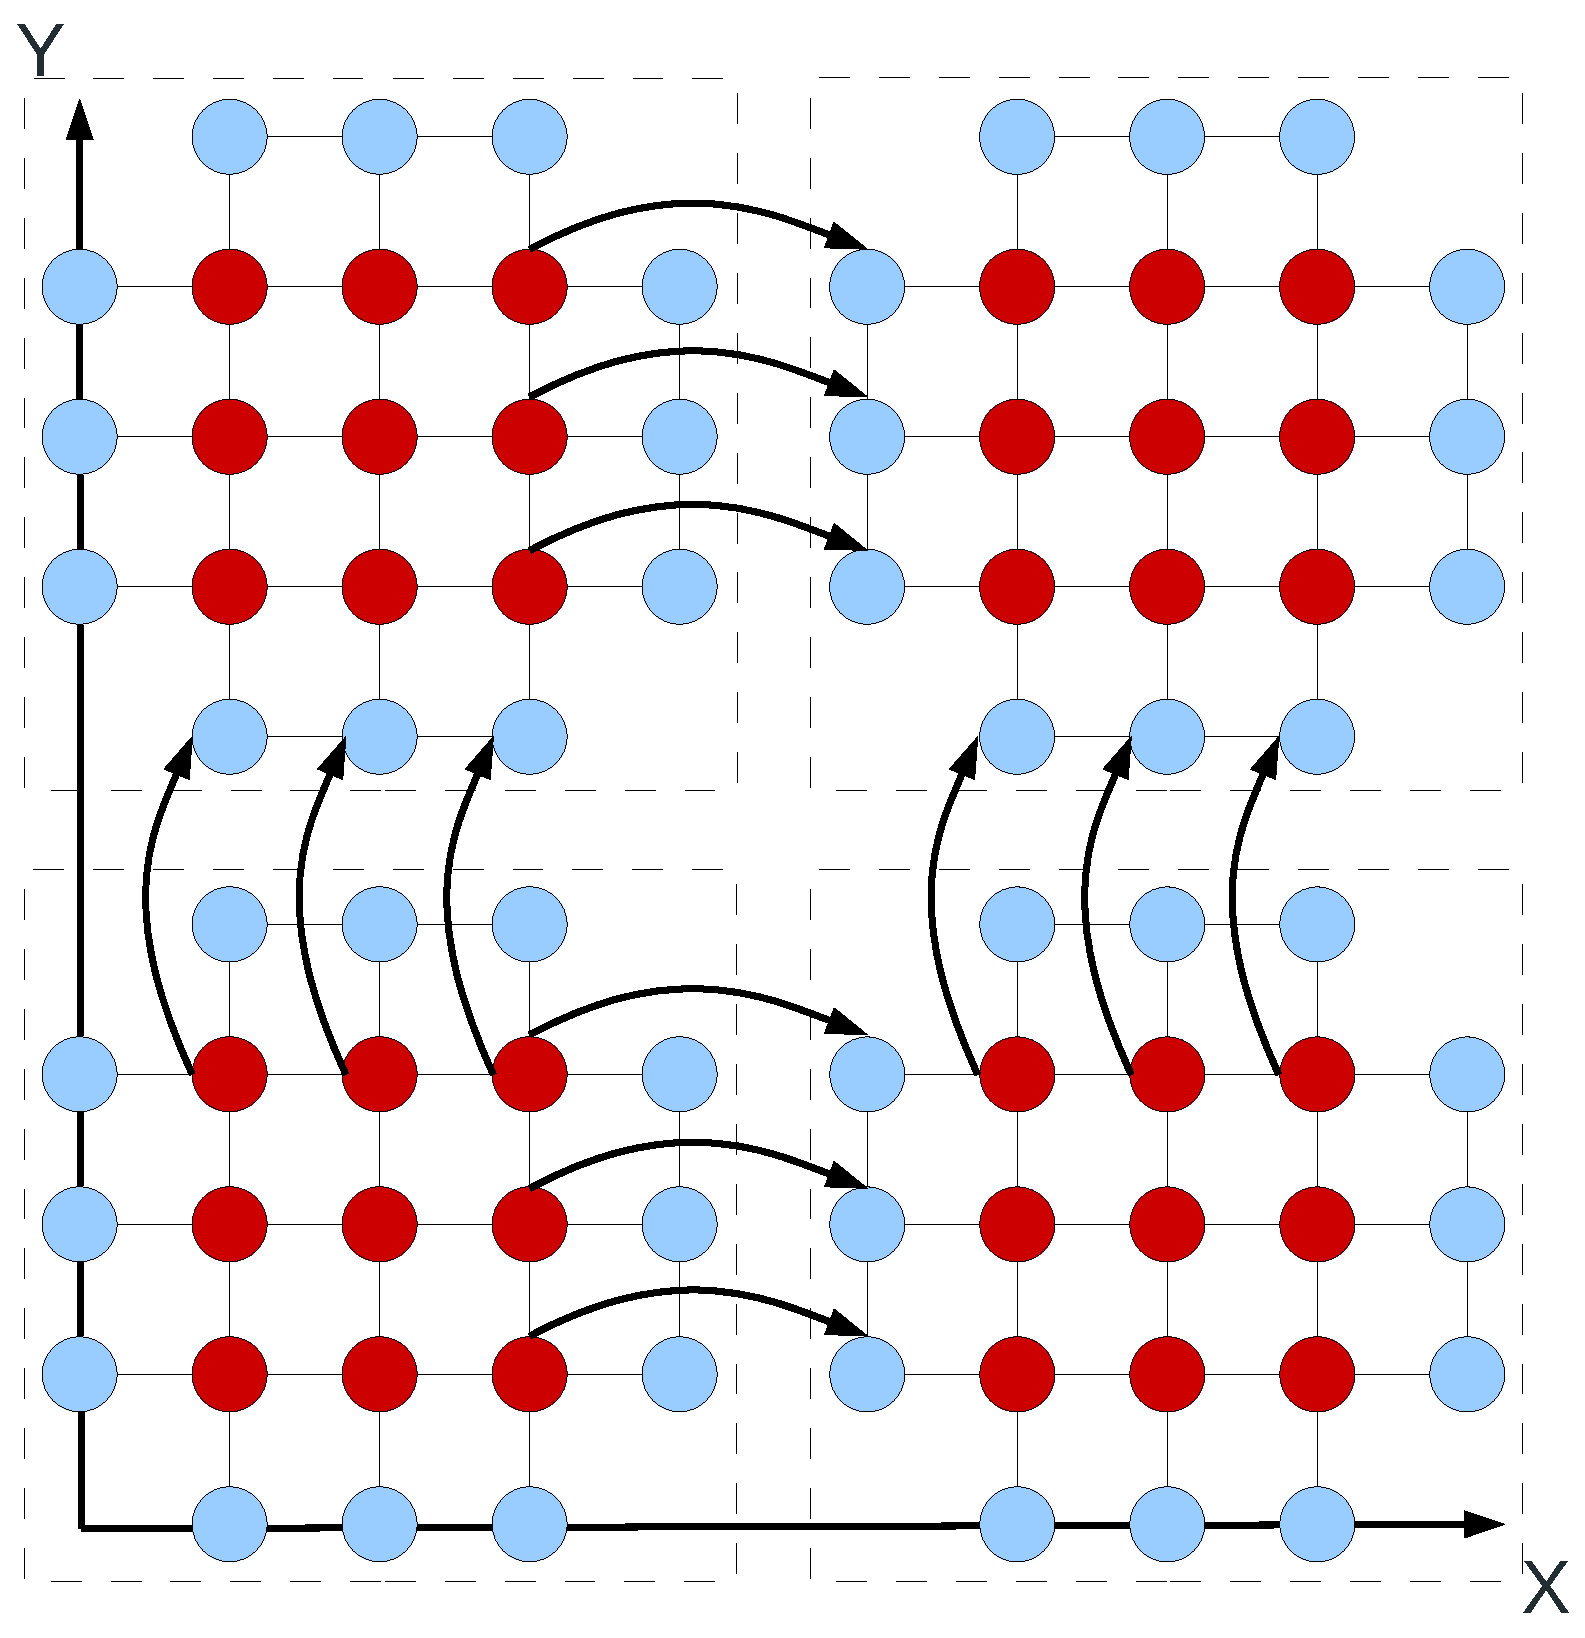
\includegraphics[height=2.5in]{artwork/pdf/decomp_3}
\end{figure}

\end{frame}


\begin{frame}{Синхронизация граничных узлов}

\begin{figure}
\centering
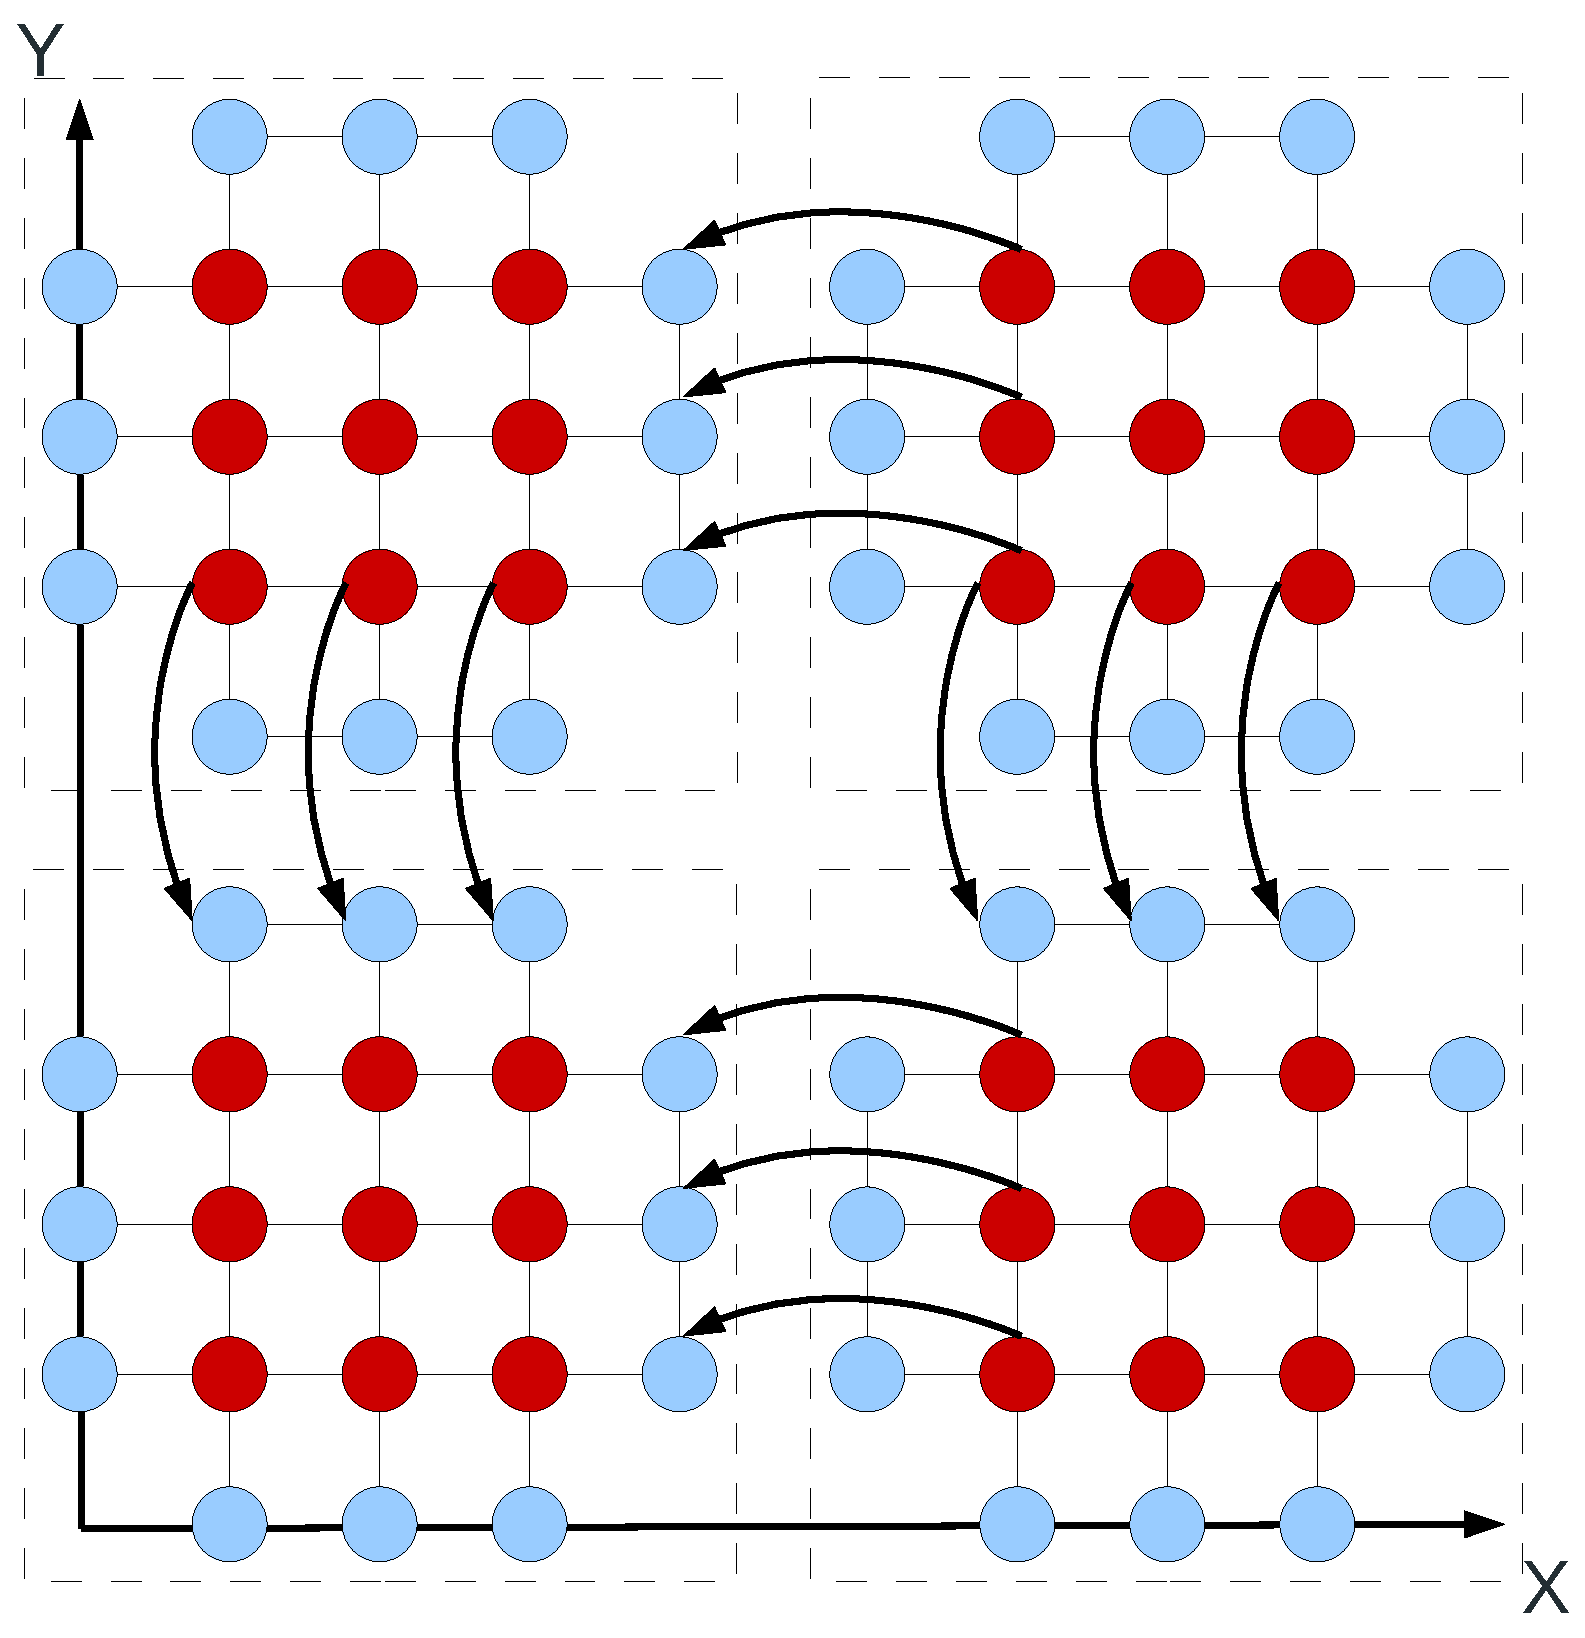
\includegraphics[height=2.5in]{artwork/pdf/decomp_4}
\end{figure}

\end{frame}
\begin{frame}{Заключение}

\begin{itemize}
   \item Изучена предметная область численных решений уравнения адвекции
   \item Протестирована последовательная версия алгоритма MPDATA
   \item Начата разработка CUDA реализации алгоритма MPDATA
   \item Реализована проблемно-независимая распределенная среда обмена границами
\end{itemize}

\end{frame}



\bibliographystyle{abbrv}
\bibliography{library}

\end{document}

